\documentclass[a4paper]{article}

\usepackage{amsfonts}
\usepackage[francais,english]{babel}
\usepackage[T1]{fontenc}
\usepackage[]{fullpage}
\usepackage{graphicx}
\usepackage{hyperref}
\usepackage[utf8]{inputenc}
\usepackage{subfigure}

\makeatletter
\def\thickhrulefill{\leavevmode \leaders \hrule height 1pt\hfill \kern \z@}
\def\maketitle{%
  \null
  \thispagestyle{empty}%
  \vskip 1cm
  \begin{flushright}
        \normalfont\Large\@author
  \end{flushright}
  \vfil
  \hrule height 2pt
  \par
  \begin{center}
        \huge \strut \@title \par
  \end{center}
  \hrule height 2pt
  \begin{center}
  		$7$ Mars $2013$
  \end{center}
  \par
  \vfil
  \vfil
  \null
\begin{center}
\Huge{Placement constraints for a better QoS in clouds}
\end{center}
\begin{figure}[!ht]
	\centering
	
\includegraphics[scale=.45]{imgs/cloud.png}
\end{figure}
\vfil
\begin{figure}[!ht]
	\centering
	
\includegraphics[scale=.5]{imgs/polytech.png}
\end{figure}
\vfil
\begin{description}
	\item[Entreprise] Université de Nice-Sophia Antipolis
	\item[Lieu] Sophia-Antipolis, France
	\item[Responsable] Fabien Hermenier, équipe OASIS,
		\href{mailto:fabien.hermenier@unice.fr}{fabien.hermenier@unice.fr}
\end{description}
\cleardoublepage
}
\makeatother
\author{Mathieu Bivert, CSSR, \href{mailto:bivert@essi.fr}{bivert@essi.fr}}
\title{PFE : Rendu intérmédiaire $D_2$}

\begin{document}
\maketitle

\selectlanguage{francais}
	\begin{abstract}
		Ce document présente une formalisation du typage des nœuds
		et des machines virtuelles dans le cadre du logiciel Entropy.
		Une implémentation y est décrite succintement.
	\end{abstract}

\selectlanguage{english}
	\begin{abstract}
		This document describes a formalisation of the nodes and virtual
		machines typing within the framework of Entropy. A implementation
		is also succintly described.
	\end{abstract}

\selectlanguage{francais}

\tableofcontents
\newpage

\section{Introduction}
\subsection{Généralités et vocabulaire}
BtrPlace est un logiciel permettant de répartir efficacement un ensemble
de machines virtuelles (VMs) sur un ensemble de nœuds en respectant un ensemble
de contraintes donnés par l'utilisateur. Pour ce faire, BtrPlace modélise les
actions sur les VMs et nœuds (comme l'éteignage, l'allumage, etc.) via des intervalles
de durées appellés slices. Le but de cette partie du travail est de typer VMs et nœuds, afin de refléter les différents hyperviseurs présents sur le marché.

Plus formellement:
\begin{description}
	\item[Type] entier $t \in \mathcal T$ associé à chaque système de virtualisation,
		par exemple, KVM$=0$, VMWare$=1$, \ldots
	\item[Nœud] serveur physique, noté $n \in \mathcal N$,doté d'un
		type courant $T(n)$ et d'un ensemble de types possibles
		$\mathcal{T}_n$;
	\item[VM] machine virtuelle, notée $v \in \mathcal V$, à laquelle
		est associée un type fixe $T(v) \in \mathcal T$ et un emplacement courant $P(v) \in \mathcal N$;
	\item[Déploiement] opération de redémarrage de nœud, éventuellement
		accompagnée d'un changement de type pour le nœud.
	\item[Reconfiguration] opération durant laquelle BtrPlace change le
		placement des VMs sur les nœuds, en fonction des contraintes
		établies par l'utilisateur;
	\item[Slices] la modélisation des actions de reconfiguration~\cite{herm2012}
		est réalisée à l'aide de \textit{slices}, qui correspondent à
		une durée finie pendant un processus de reconfiguration, durant laquelle
		des ressources sont utilisées. Il existe deux types de slices:
	\begin{description}
		\item[consuming slice], $c \in \mathcal C$, où les ressources sont
			utilisées au début de la reconfiguration;
		\item[demanding slice], $d \in \mathcal D$, où les ressources sont
		utilisées à la fin de la reconfiguration;
	\end{description}
\end{description}

La fonction $T$ associe à une VM ou un nœud son type; la fonction $P$
associe à une VM ou une slice un nœud.

Un nœud est doté d'une nouvelle dimension de type. Celle-ci
est booléenne : soit le type change, auquel cas, la valeur est de $1$,
sinon, elle vaut $0$. Dans les graphes suivants, elle est représentée
à part pour des questions de lisibilité.

\subsection{Configuration d'exemple}
Dans un premier temps, nous cherchons à obtenir une configuration minimaliste,
mettant en œuvre suffisamment d'éléments pour représenter le problème:
\begin{figure}[!ht]
	\centering
	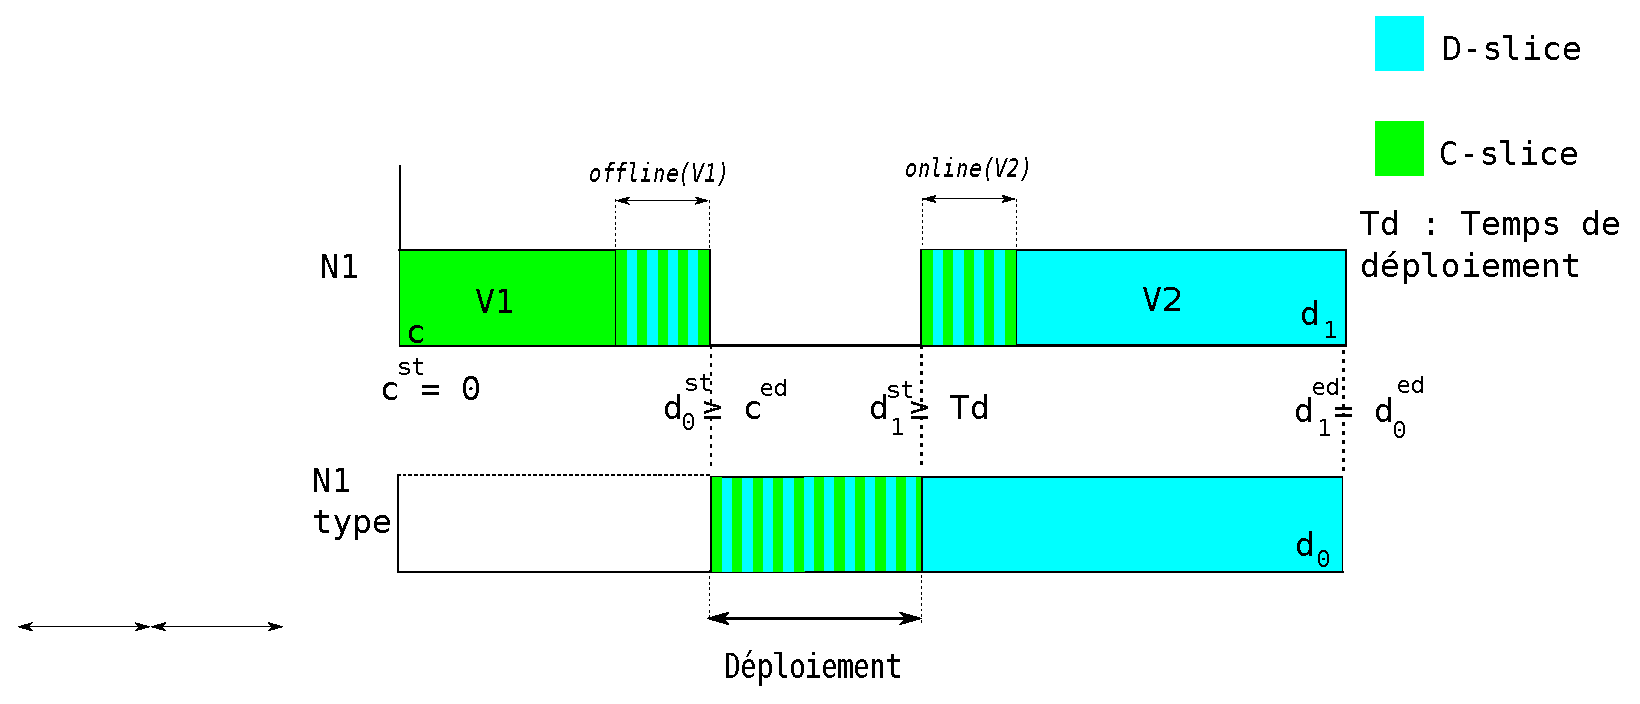
\includegraphics[scale=.45]{imgs/config.eps}
	\caption{\label{config} Exemple de configuration mettant en œuvre un
		changement de type; $v_1$ est mise hors-ligne, $v_2$ est allumée}
\end{figure}

Sur la figure \ref{config}, $v_1$ et $v_2$ sont deux machines
virtuelles de types différents, par exemple Xen et VMWare.
Pour simplifier le problème, seules les actions de démarrage et d'éteignage
pour les VMs sont prises en compte. En effet, considérer
d'autres types d'actions dans cet exemple ne change pas le
problème, la modélisation par des slices permettant de s'abstraire
des actions précises sur VMs.

L'opération de déploiement sur le nœud $n_1$ se résume à:
\begin{enumerate}
	\item s'assurer que toutes les VMs présentent sur $v_1$ sont migrées;
	\item mettre hors-ligne $v_1$;
	\item éteindre $n_1$;
	\item allumer $n_1$ en changeant son type, c'est-à-dire en changeant
		son hyperviseur.
	\item démarrer $v_2$;
\end{enumerate}
Le temps $T_d$ pris par cette opération est spécifié par l'admninistrateur
du datacenter dans la configuration de BtrPlace.

Dans les paragraphes qui suivent, nous cherchons un modèle correspondant
à l'exemple du paragraphe précèdent. Nous commencons par décrire cas général,
puis nous travaillons par incrément depuis un cas particulier pour arriver à une
implémentation « complète ».

\section{Modélisation abstraite du cas général}
Une variable est associée à chaque type de plateforme.
Pour chaque type de plateforme, une dimension est ajoutée à chaque
nœud. Ces variales sont stockées dans un vecteur
$v \in \mathbb{N}^n$. La façon dont $v$ est construit et la justification
de l'ensemble de définition des dimensions ($\mathbb{N}$) sont données
dans la section suivante.

Le placement est satisfait ssi au plus une seule de ces dimensions est
non nulle:
\[
	(\exists ! x \in v_i), x \neq 0\ (0)
\]

La contrainte est donc satisfaite pour un nœud $n$ dans deux cas:
\begin{enumerate}
	\item $v_i$ ne contient que des $0$ : aucun hyperviseur n'est actif;
	\item $v_i$ a une composante non-nulle : un unique hyperviseur tourne sur $n$.
\end{enumerate}

\section{Modélisation pour BtrPlace}
\subsection{Cas général}
Pour construire les vecteurs $v_i$, les nœuds utilisés dans le
processus de reconfiguration sont parcourus pour créer une table recensant les
différents types d'hyperviseurs. L'utilisation d'une table permet de coder
les chaînes de caractères décrivant les hyperviseurs afin de pouvoir les
utiliser dans BtrPlace.

Dans le cas présent, la dimension $d=v_i$ peut très bien être de type booléene:
si le nœud supporte le type, $d$ est vraie, sinon $d$ est fausse.
Cependant, les licences d'utilisations des hyperviseurs spécifient
parfois un nombre limités de machines virtuelles pouvant tourner. Afin
de prendre en compte ce cas, il est intéressant d'utiliser une dimension
entière, représentant le nombre de machines virtuelles de type $t$
autorisées à fonctionner sur le nœud. C'est le cas pour les produits
VMWare\footnote{\url{https://www.vmware.com/support/licensing/per-vm/}}.
Des limitations pour d'autres ressources (RAM, NIC, etc.) existent pour
XenServer\footnote{\url{http://support.citrix.com/article/CTX134887\#P98\_7562}},
ce qui laisse sous-entendre que la modélisation utilisée ici pourrait
être utilisée pourrait être étendue.

L'équation $(0)$ est équivalente à l'équation suivante, exprimée en terme
de contraintes:
\[
	OccurenceMin(v_i, 0) == len(v_i)-1
	\Leftrightarrow
	Occurence((v_i:len(v_i)-1, 0, true, true)
\]

\textit{OccurenceMin} est deprecated mais tout de même présenté cas plus
simple qu'\textit{Occurence}. Des détails sur ce dernier sont fournis
dans la section implémentation.

\subsection{Cas particulier : le nouveau type d'une plateforme est connu}
Lorsque le nouveau type est une propriété du modèle qui n'a pas à être
déterminée par le solveur, le problème peut être simplifié. L'utilisation
d'une slice pour la dimension de temps devient inutile; deux variables indiquant
les temps de début et de fin de l'opération de déploiement, respectivement notés $D^\mathrm{st}$ et $D^\mathrm{ed}$, sont suffisantes.

Le type du nœud étant modifié, les VMs présentes au début de la reconfiguration
doivent nécessairement être déplacées ou migrées, suivant les autres
contraintes. Les nouvelles VMs peuvent alors être placées à l'aide de
la contrainte \textit{fence}, d'une façon similaire à ce qui se passe dans
\textit{StaticPlatform.java}\footnote{\url{https://github.com/Heaumer/pfe/blob/master/entropy-fh/src/main/java/entropy/plan/choco/constraint/platform/StaticPlatform.java}}.
\textit{Fence} contraint un ensemble de VMs à tourner sur un
ensemble de nœuds; donc dans le cas présent, limite le placement des VMs
au nœuds ayant le même type.

Pour satisfaire le placement sur un nœud $n$, deux contraintes supplémentaires sont
données au solveur:

\begin{enumerate}
	\item Les anciennes VMs partent avant le début de l'opération de
		redéploiement, c'est-à-dire,
\[
	(\forall c \in \mathcal C), P(c) = n \Rightarrow c^\mathrm{ed} \leq D^\mathrm{st}
\]
	\item Les nouvelles VMs arrivent une fois le redéploiement terminé,
		c'est-à-dire:
\[
	(\forall d \in \mathcal D), P(d) = n \Rightarrow d^\mathrm{st} \geq D^\mathrm{ed}
\]
\end{enumerate}
Le placement est satisfait ssi chaque VM est bien placée sur
un nœud de même type, ie.:
\[
	(\forall v \in \mathcal V), (\exists n \in \mathcal N), P(v) = n
		\Rightarrow T(n) = T(v)	
\]

Cette contrainte doit être implémentée dans BtrPlace via Choco.

\section{Implémentation}
\subsection{Retypage}
Afin de gérer le changement d'hyperviseur, une nouvelle action est requise.
La classe \textit{Retype}\footnote{\url{https://github.com/Heaumer/pfe/blob/master/entropy-fh/src/main/java/entropy/plan/action/Retype.java}}, qui est
une action de type \textit{Startup}, permet de retyper un nœud. 
Successivement, elle
\begin{enumerate}
	\item créee une copie du nœud;
	\item le supprime de la configuration;
	\item change l'hyperviseur de la copie du nœud;
	\item ajoute la copie dans la configuration.
\end{enumerate}

Un nouvel action model \textit{RetypeNodeActionModel}\footnote{\url{https://github.com/Heaumer/pfe/blob/master/entropy-fh/src/main/java/entropy/plan/choco/actionModel/RetypeNodeActionModel.java}}
modèlise le changement de type au sein de choco, en ajoutant successivement
une action de \textit{Shutdown} puis de \textit{Retype} pour éteindre et
changer l'hyperviseur d'un nœud. Le constructeur de cet action model prends
en paramètres, en plus du nœud à retyper et son nouveau type, le début de
l'action d'éteignage du nœud, et le début du retypage.

Enfin, l'implémentation de \textit{DefaultReconfigurationProblem} se charge
d'instancier cet action model en cas de changement de type.

\subsection{Cas particulier}
\begin{verbatim}
Interface: Platform({ nœud_i -> plateforme, nœud_j -> plateforme, …})
\end{verbatim}

Une nouvelle contrainte de placement \textit{Platform} est ajoutée. Son
constructeur prends en argument une \textit{HashMap} associant les
nœuds devant changer de type à leur nouvelle plateforme.

Les VMs présentent sur le nœud sont alors contraintes à se déplacer
avant le temps de début de redémarrage du serveur. Pour ce faire,
cette contrainte de temps est mise sur les c-slices des actions
associées à ces VMs.

Enfin, si le nœud s'apprête à changer de type, parmi les
d-slices entrant en jeu dans la reconfiguration, celles dont
les les VMs associées ont le même type que le nœud à la fin du processus
sont sélectionnées. Finalement, ces slices sont contraintes à ne démarrer
qu'après la fin du processus de retypage, c'est-à-dire une fois que
le nœud a bien redémarré et changé d'hyperviseur.

Le code implémentant la contrainte est
disponible\footnote{\url{https://github.com/Heaumer/pfe/blob/master/entropy-fh/src/main/java/entropy/vjob/Platform.java}}. Cette
classe est testée\footnote{\url{https://github.com/Heaumer/pfe/blob/master/entropy-fh/src/test/java/entropy/vjob/constraint/TestPlatform.java}}
en suivant des use-cases définis par Fabien Hermenier.

\subsection{Cas général}
De même que pour le cas particulier, une nouvelle contrainte
\textit{TypedPlatform}\footnote{\url{https://github.com/Heaumer/pfe/blob/master/entropy-fh/src/main/java/entropy/vjob/TypedPlatform.java}}
est ajoutée. Le constructeur prends en argument un ensemble de nœuds
à typer. Pour chaque nœud, la contrainte s'assure qu'au plus, un
unique élément du vecteur contenant les plateformes possibles est non
null. Pour ce faire, la classe \textit{Occurence} de choco est
utilisée : 
La documentation d'\textit{Occurence}:
\begin{verbatim}
public Occurrence(IntDomainVar[] vars,
                  int occval,
                  boolean onInf,
                  boolean onSup)
\end{verbatim}
Dans notre cas, le dernier élément de \textit{vars} contient le nombre
minimum de \textit{occval}$=0$ devant être présents dans le reste du
tableau \textit{vars[]}.
Par manque de temps, cette classe n'est pas testée.

\section{Validation}
Les implémentations précèdentes sont validées pas des tests unitaires mettant
en œuvre des uses-cases significatifs vus avec l'encadrant.
\subsection{Cas particulier (contrainte \textit{Platform})}
\subsubsection{Sans changement de type}
Soient un nœud $n_1$ supportant un unique hyperviseur $h_1$, et deux
machines virtuelles $v_1$ et $v_2$, de types respectifs $h_1$ et $h_2$.
La consommation en ressource de $v_1$ comme de $v_2$ est inférieure aux
possibilités offertes par $n_1$.

Il faut alors s'assurer que placer:
\begin{itemize}
	\item $v_1$ sur $n_1$ satisfait bien la contrainte \textit{Platform};
	\item $v_2$ sur $n_1$ ne satisfait pas la contrainte.
\end{itemize}
\subsubsection{Type variable}
Soient deux nœuds $n_1$ et $n_2$ supportant respectivement les hyperviseurs
$h_1, h_2$ et $h_1$. Soient deux machines virtuelles $v_1$ et $v_2$ de
types respectifs $h_1$ et $h_2$. Au début du processus de reconfiguration,
les deux nœuds tournent sous $h_1$; $v_1$ tourne sur $n_1$ et $v_2$ est
éteinte. À la fin, $n_1$ aura changé son type d'hyperviseur à $h_2$, et
$v_2$ doit être allumée.

\subsection{Cas général}
Comme mentionné dans la section précèdente, cette classe n'a pas été testée.
\newpage
\selectlanguage{francais}
\bibliographystyle{alpha}
\bibliography{docs}

\end{document}
